
\section{DIM approach: a mean-field description of the interaction between K and $^4$He$_N$}

\subsection{General principle}

So far, we have discussed how to deal with a pure helium droplet.
In order to describe the full KHe$_N$ system, we now turn to the interaction part.
The following discussion will be presented in a quite general way.\\

The total interaction of K with the droplet is approximated by a sum of pair-wise diatomic interactions.
This is justified since He is a rare gas atom and the K-He interaction is weak.
The validity of this approximation (and of the pair-wise potentials used) is tested by calculating the absorption spectra, see \citsec{sec:4P-spectra}.
This is the so-called \textit{Diatomic In Molecules} (DIM) model \cite{Ell63}. 
We first describe the case of a single KHe diatomic and then move on to the KHe$_N$ interaction.

\subsection{The diatomic case: K-He}

\label{sec:DIM-dia}
		
The standard \textsc{Born-Oppenheimer} approximation states that the fast electronic motion of electrons can be decoupled from the slow nuclei one. 
From a mathematical point of view, one has to solve the \textsc{Schr\"odinger} equation for the motion of the electrons for fixed nuclei positions treated as parameters (so-called \emph{electronic \textsc{Schr\"odinger} equation)}.
This results in a set of eigenvalues $V_\beta(\textbf{r})$ which constitute the interaction potentials  between nuclei in the different possible electronic states labeled with $\{\beta\}$ as quantum numbers. \\

Potassium is an alkali, hence it can be described as a one active electron system. 
We introduce different operators that will be useful to characterize its electronic states: 
orbital ($\vb{L}$), spin ($\vb{S}$) and total ($\vb{J} = \vb{L}+ \vb{S}$) angular momentum, that actually refers to the single electron.
In particular, we will be using three different quantum numbers (others than $n$ and $l$): $\Lambda$ ($L_z$), $\Omega$ ($J_z$) and $J$ ($\vb{J}^2$), where $z$ is the internuclear axis.\\

Because of cylindrical symmetry, $L_z$ commutes with the electronic Hamiltonian (in the absence of spin-orbit coupling) and $\Lambda$ is then a good quantum number.
Even though the atomic quantum numbers $n$ and $l$ are mixed in principle, the interaction with helium is rather weak and we can consider effective $(nl)$ orbitals to describe the subspace of electronic states going asymptotically to He + K$(nl)$.
No analytical expression is obtained for the radial components as it is not needed, but the angular part is assumed to be the usual spherical harmonics orbitals.
Moreover, for computing facilities, we will be working in the basis set of ``real spherical harmonics'' (combinations of $Y_{l,\pm\Lambda}$, which implies to change basis when including spin-orbit coupling). \\

Our study involves three different $nl$-states: ($4s$), ($4p$) and ($5s$). 
Let us first neglect spin-orbit coupling. 
While the $s$-state interaction is simple, the $p$-state one splits into two different states with $\Lambda$ as a good quantum number. 
\begin{figure}[h!]
\centering
    % GNUPLOT: LaTeX picture with Postscript
\begingroup
  \makeatletter
  \providecommand\color[2][]{%
    \GenericError{(gnuplot) \space\space\space\@spaces}{%
      Package color not loaded in conjunction with
      terminal option `colourtext'%
    }{See the gnuplot documentation for explanation.%
    }{Either use 'blacktext' in gnuplot or load the package
      color.sty in LaTeX.}%
    \renewcommand\color[2][]{}%
  }%
  \providecommand\includegraphics[2][]{%
    \GenericError{(gnuplot) \space\space\space\@spaces}{%
      Package graphicx or graphics not loaded%
    }{See the gnuplot documentation for explanation.%
    }{The gnuplot epslatex terminal needs graphicx.sty or graphics.sty.}%
    \renewcommand\includegraphics[2][]{}%
  }%
  \providecommand\rotatebox[2]{#2}%
  \@ifundefined{ifGPcolor}{%
    \newif\ifGPcolor
    \GPcolortrue
  }{}%
  \@ifundefined{ifGPblacktext}{%
    \newif\ifGPblacktext
    \GPblacktextfalse
  }{}%
  % define a \g@addto@macro without @ in the name:
  \let\gplgaddtomacro\g@addto@macro
  % define empty templates for all commands taking text:
  \gdef\gplbacktext{}%
  \gdef\gplfronttext{}%
  \makeatother
  \ifGPblacktext
    % no textcolor at all
    \def\colorrgb#1{}%
    \def\colorgray#1{}%
  \else
    % gray or color?
    \ifGPcolor
      \def\colorrgb#1{\color[rgb]{#1}}%
      \def\colorgray#1{\color[gray]{#1}}%
      \expandafter\def\csname LTw\endcsname{\color{white}}%
      \expandafter\def\csname LTb\endcsname{\color{black}}%
      \expandafter\def\csname LTa\endcsname{\color{black}}%
      \expandafter\def\csname LT0\endcsname{\color[rgb]{1,0,0}}%
      \expandafter\def\csname LT1\endcsname{\color[rgb]{0,1,0}}%
      \expandafter\def\csname LT2\endcsname{\color[rgb]{0,0,1}}%
      \expandafter\def\csname LT3\endcsname{\color[rgb]{1,0,1}}%
      \expandafter\def\csname LT4\endcsname{\color[rgb]{0,1,1}}%
      \expandafter\def\csname LT5\endcsname{\color[rgb]{1,1,0}}%
      \expandafter\def\csname LT6\endcsname{\color[rgb]{0,0,0}}%
      \expandafter\def\csname LT7\endcsname{\color[rgb]{1,0.3,0}}%
      \expandafter\def\csname LT8\endcsname{\color[rgb]{0.5,0.5,0.5}}%
    \else
      % gray
      \def\colorrgb#1{\color{black}}%
      \def\colorgray#1{\color[gray]{#1}}%
      \expandafter\def\csname LTw\endcsname{\color{white}}%
      \expandafter\def\csname LTb\endcsname{\color{black}}%
      \expandafter\def\csname LTa\endcsname{\color{black}}%
      \expandafter\def\csname LT0\endcsname{\color{black}}%
      \expandafter\def\csname LT1\endcsname{\color{black}}%
      \expandafter\def\csname LT2\endcsname{\color{black}}%
      \expandafter\def\csname LT3\endcsname{\color{black}}%
      \expandafter\def\csname LT4\endcsname{\color{black}}%
      \expandafter\def\csname LT5\endcsname{\color{black}}%
      \expandafter\def\csname LT6\endcsname{\color{black}}%
      \expandafter\def\csname LT7\endcsname{\color{black}}%
      \expandafter\def\csname LT8\endcsname{\color{black}}%
    \fi
  \fi
    \setlength{\unitlength}{0.0500bp}%
    \ifx\gptboxheight\undefined%
      \newlength{\gptboxheight}%
      \newlength{\gptboxwidth}%
      \newsavebox{\gptboxtext}%
    \fi%
    \setlength{\fboxrule}{0.5pt}%
    \setlength{\fboxsep}{1pt}%
\begin{picture}(5760.00,1440.00)%
    \gplgaddtomacro\gplbacktext{%
      \csname LTb\endcsname%
      \put(415,720){\makebox(0,0)[r]{\strut{}$\Pi (\Lambda=\pm1$)}}%
      \put(5275,720){\makebox(0,0)[l]{\strut{}$\Sigma (\Lambda=0)$}}%
    }%
    \gplgaddtomacro\gplfronttext{%
    }%
    \gplbacktext
    \put(0,0){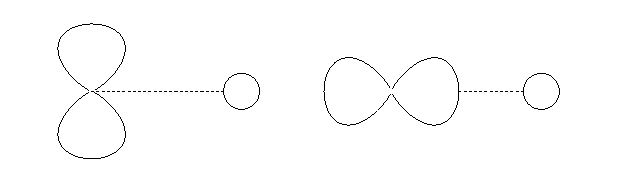
\includegraphics{DIM-p-splitting}}%
    \gplfronttext
  \end{picture}%
\endgroup

    \caption{Illustration and labeling of energy level splitting in K($np$) state interaction with He}
\end{figure}

We assume that spin-orbit coupling is the same that in free atom ($A_\LS$ for free K from \cite{Nist})
\begin{align}
H^{nl/\SO} = A_\LS \, \vb{L}\cdot\vb{S} \label{eq:DIM-HSO}
\end{align}
We know that $s$-states are not affected (they are just doubly degenerated since $S=1/2$), but $p$-states get an additional energy splitting, with good quantum number $\Omega$ (because $J_z=L_z+S_z$ obviously commutes with the spin-orbit Hamiltonian but also with the electrostatic interaction one since $L_z$ (and $S_z$) do). 
It is therefore important to note that when electrostatic interaction is large \textit{id est} at short distances then $\Lambda$ is almost a good quantum number and in the opposite way at large distances it is $J$. \\

In practice we start from \textsc{Pascale} \cite{Pas1983} $V^{4p}_\Sigma(\vb{r})$, $V^{4p}_\Pi(\vb{r})$, $V^{5s}(\vb{r})$ and \textsc{Patil} \cite{Pat1991} $V^{4s}(\vb{r})$ pair potentials that do not include spin-orbit coupling.
The electrostatic interaction is expressed as
\begin{itemize}
\item for the ground state: $(4s)$
\begin{align}
H^{4s}(\vb{r}) = V^{4s}(\vb{r}) \ket{4s}\bra{4s} 
\label{eq:DIM-pair-pot-4s}
\end{align}
\item for the first excited $p$-state: $(4p)$
\begin{align*}
H^{4p}(\vb{r}) %&= \mqty(\dmat[0]{V_\Pi^{4p}(\vb{r}),V_\Pi^{4p}(\vb{r}),V^{4p}_\Sigma(\vb{r})}) \\
&=V_\Pi^{4p}(\vb{r})\{\ket{4p_x}\bra{4p_x}+\ket{4p_y}\bra{4p_y} \} + V^{4p}_\Sigma(\vb{r}) \ket{4p_z}\bra{4p_z} \\
&=V_\Pi^{4p}(\vb{r}) \cdot \mathbb{I}_3 + [V^{4p}_\Sigma(\vb{r}) - V^{4p}_\Pi(\vb{r})] \ket{4p_z}\bra{4p_z} \label{eq:DIM-pair-pot-4p} \num
\end{align*}
\item for the first excited $s$-state: $(5s)$
\begin{align}
H^{5s}(\vb{r}) = V^{5s}(\vb{r}) \ket{5s}\bra{5s}
\label{eq:DIM-pair-pot-5s}
\end{align}
\end{itemize}

The total electronic Hamiltonian is then written as the sum of the electrostatic interaction denoted ES and the spin orbit coupling denoted SO
\begin{align}
H^{nl}_\KHE &= H^{nl/\DIM}_\KHE + H^{nl/\SO} = H^{nl/\DIM}_\KHE + A_\LS \, \vb{L}\cdot\vb{S} = H^{nl/\DIM}_\KHE + \frac{A_\LS}{2}(\vb{J}^2-\vb{L}^2-\vb{S}^2)
\end{align}

\subsection{DIM and mean-field theory}

We need to introduce a set of orbitals as a basis for our study. We choose the \textbf{uncoupled basis of real orbitals oriented along the pseudo-internuclear axis} (\citfig{fig:DIM-axis}) denoted $\{\ket{nl_i,\pm}\}$, where $nl_i$ refers to the $i$-th spatial orbital associated with the ($nl$) state and $\pm$ refers to the spin state (actually $\pm 1/2$ since $S=1/2$). For instance in the $nl=4p$ case, the basis is $\{\ket{4p_x,\pm}, \ket{4p_y,\pm}, \ket{4p_z,\pm} \}$, while for $ns$ states the basis is $\{\ket{ns,\pm}\}$.
As we already said: the principle of this approach is to write the total electrostatic Hamiltonian as the sum over all pair contributions 
\begin{align}
H^{nl}_\KHEN &= \sum_{m=1}^{m=N} H^{nl/\DIM}_\KHE(\vb{r}_m) + H^{nl/\SO} \equiv H^{nl/\DIM}_\KHEN + H^{nl/\SO}\label{eq:DIM-hamtot}
\end{align}
%
\begin{figure}[h!]
%\hspace{-\oldindent}
\begin{minipage}[c]{.55\linewidth}
\hspace{\oldindent}
Here is a tricky point:  the $m$-th pair-interaction Hamiltonian in (\ref{eq:DIM-hamtot}) is actually expressed in a set of orbitals defined in the axes attached to the $m$-th internuclear axis, but we want this one to be expressed in the previously chosen basis, common to all pairs.
We then need to express those pair Hamiltonians in the common basis.
This is done by applying a rotation $\mathcal{R}_m:\hat{\vb{z}}_m \longmapsto  \hat{\vb{z}} \propto \vb{r}_\K$ (which depends on the angular momentum)
\begin{align}
H^{nl/\DIM}_\KHEN &= \sum_{m=1}^{m=N} \mathcal{R}_m^{-1} H^{nl/\DIM}_\KHE(\vb{r}_m) \, \mathcal{R}_m
\end{align}
\end{minipage} \hfill
\begin{minipage}[c]{.40\linewidth} 
\rotatebox{-90}{% GNUPLOT: LaTeX picture with Postscript
\begingroup
  \makeatletter
  \providecommand\color[2][]{%
    \GenericError{(gnuplot) \space\space\space\@spaces}{%
      Package color not loaded in conjunction with
      terminal option `colourtext'%
    }{See the gnuplot documentation for explanation.%
    }{Either use 'blacktext' in gnuplot or load the package
      color.sty in LaTeX.}%
    \renewcommand\color[2][]{}%
  }%
  \providecommand\includegraphics[2][]{%
    \GenericError{(gnuplot) \space\space\space\@spaces}{%
      Package graphicx or graphics not loaded%
    }{See the gnuplot documentation for explanation.%
    }{The gnuplot epslatex terminal needs graphicx.sty or graphics.sty.}%
    \renewcommand\includegraphics[2][]{}%
  }%
  \providecommand\rotatebox[2]{#2}%
  \@ifundefined{ifGPcolor}{%
    \newif\ifGPcolor
    \GPcolortrue
  }{}%
  \@ifundefined{ifGPblacktext}{%
    \newif\ifGPblacktext
    \GPblacktextfalse
  }{}%
  % define a \g@addto@macro without @ in the name:
  \let\gplgaddtomacro\g@addto@macro
  % define empty templates for all commands taking text:
  \gdef\gplbacktext{}%
  \gdef\gplfronttext{}%
  \makeatother
  \ifGPblacktext
    % no textcolor at all
    \def\colorrgb#1{}%
    \def\colorgray#1{}%
  \else
    % gray or color?
    \ifGPcolor
      \def\colorrgb#1{\color[rgb]{#1}}%
      \def\colorgray#1{\color[gray]{#1}}%
      \expandafter\def\csname LTw\endcsname{\color{white}}%
      \expandafter\def\csname LTb\endcsname{\color{black}}%
      \expandafter\def\csname LTa\endcsname{\color{black}}%
      \expandafter\def\csname LT0\endcsname{\color[rgb]{1,0,0}}%
      \expandafter\def\csname LT1\endcsname{\color[rgb]{0,1,0}}%
      \expandafter\def\csname LT2\endcsname{\color[rgb]{0,0,1}}%
      \expandafter\def\csname LT3\endcsname{\color[rgb]{1,0,1}}%
      \expandafter\def\csname LT4\endcsname{\color[rgb]{0,1,1}}%
      \expandafter\def\csname LT5\endcsname{\color[rgb]{1,1,0}}%
      \expandafter\def\csname LT6\endcsname{\color[rgb]{0,0,0}}%
      \expandafter\def\csname LT7\endcsname{\color[rgb]{1,0.3,0}}%
      \expandafter\def\csname LT8\endcsname{\color[rgb]{0.5,0.5,0.5}}%
    \else
      % gray
      \def\colorrgb#1{\color{black}}%
      \def\colorgray#1{\color[gray]{#1}}%
      \expandafter\def\csname LTw\endcsname{\color{white}}%
      \expandafter\def\csname LTb\endcsname{\color{black}}%
      \expandafter\def\csname LTa\endcsname{\color{black}}%
      \expandafter\def\csname LT0\endcsname{\color{black}}%
      \expandafter\def\csname LT1\endcsname{\color{black}}%
      \expandafter\def\csname LT2\endcsname{\color{black}}%
      \expandafter\def\csname LT3\endcsname{\color{black}}%
      \expandafter\def\csname LT4\endcsname{\color{black}}%
      \expandafter\def\csname LT5\endcsname{\color{black}}%
      \expandafter\def\csname LT6\endcsname{\color{black}}%
      \expandafter\def\csname LT7\endcsname{\color{black}}%
      \expandafter\def\csname LT8\endcsname{\color{black}}%
    \fi
  \fi
    \setlength{\unitlength}{0.0500bp}%
    \ifx\gptboxheight\undefined%
      \newlength{\gptboxheight}%
      \newlength{\gptboxwidth}%
      \newsavebox{\gptboxtext}%
    \fi%
    \setlength{\fboxrule}{0.5pt}%
    \setlength{\fboxsep}{1pt}%
\begin{picture}(2160.00,3600.00)%
    \gplgaddtomacro\gplbacktext{%
      \csname LTb\endcsname%
      \put(1560,2030){\rotatebox{90}{\makebox(0,0){\strut{}$\mathbf{r}_m$}}}%
      \put(882,1924){\rotatebox{90}{\makebox(0,0){\strut{}$\mathbf{r}_\mathrm{K}$}}}%
      \put(1467,995){\rotatebox{45}{\makebox(0,0){\strut{}$\mathbf{r}_m+\mathbf{r}_\mathrm{K}$}}}%
      \put(579,3625){\rotatebox{90}{\makebox(0,0){\strut{}$\mathbf{\hat{z}}_m$}}}%
      \put(1080,3693){\rotatebox{90}{\makebox(0,0){\strut{}$\mathbf{\hat{z}}$}}}%
    }%
    \gplgaddtomacro\gplfronttext{%
    }%
    \gplbacktext
    \put(0,0){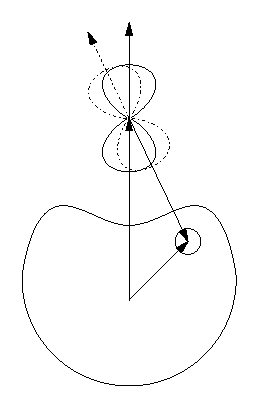
\includegraphics{DIM-axis}}%
    \gplfronttext
  \end{picture}%
\endgroup
}
\caption{Set of axes involved in our description\label{fig:DIM-axis}}
\end{minipage}
\end{figure}

We now define $U^{nl}_{ij\alpha\beta}$ which is simply the pair-interaction Hamiltonian expressed in the common basis
\begin{align}
U^{nl/\DIM}_{ij\alpha\beta}(\vb{r}_m) &= \bra{i,\alpha} \mathcal{R}_m^{-1} H^{nl/\DIM}_\KHE(\vb{r}_m) \, \mathcal{R}_m \ket{j,\beta}
\end{align}
The matrix elements of the total electrostatic Hamiltonian can then be expressed in the discrete case (helium atoms) or in the continuum case (helium density) as
\begin{align}
E^{nl/\DIM}_{ij\alpha\beta}(\{\vb{r}_m\}) &= \sum_{m=1}^{m=N} U^{nl/\DIM}_{ij\alpha\beta}(\vb{r}_m) \\
E^{nl/\DIM}_{ij\alpha\beta} (\vb{r}_\K) &= \int \dd{\vb{r}} \rho(\vb{r} + \vb{r}_\K) \, \bra{i,\alpha} \mathcal{R}^{-1}(\vb{r}) H^{nl/\DIM}_\KHE(\vb{r}) \, \mathcal{R}(\vb{r}) \ket{j,\beta} \equiv \int \dd{\vb{r}} \rho(\vb{r} + \vb{r}_\K) \, U_{ij\alpha\beta}^{nl/\DIM}(\vb{r}) \label{eq:DIM-defE}
\end{align}

\subsubsection{Spherically symmetric ($ns$) state}

Let us first consider the two ($ns$) states: ($4s$) and ($5s$). They are particularly easy to treat because the spin-orbit coupling can be omitted since $L=0$ (see \citeq{eq:DIM-HSO}). We are left with the electrostatic contribution, which is also easy to express because $s$-states are  spherically symmetric, hence invariant under rotation about they symmetry center
\begin{align*}
U^{ns/\DIM}_{ij\alpha\beta}(\vb{r}_m) &= \bra{i,\alpha} \mathcal{R}_m^{-1} H^{nl/\DIM}_\KHE(\vb{r}_m) \, \mathcal{R}_m \ket{j,\beta} \\
&= V^{ns}(\vb{r}_m) \, \bra{i,\alpha} \mathcal{R}_m^{-1} \ket{ns_m}\bra{ns_m} \, \mathcal{R}_m \ket{j,\beta} \\
&= V^{ns}(\vb{r}_m) \, \braket{i,\alpha}{ns_m}\braket{ns_m}{j,\beta} \\
&= V^{ns}(\vb{r}_m) \, \delta_{ij} \delta_{\alpha\beta}\num\\
E^{ns/\DIM}_{ij\alpha\beta} (\vb{r}_\K) &= \int \dd{\vb{r}} \rho(\vb{r} + \vb{r}_\K) \, V^{ns}(\vb{r}) \, \delta_{ij} \delta_{\alpha\beta}\num
\end{align*}

The matrix elements are clearly diagonal in the common basis $\{\ket{ns,\pm}\}$, moreover they do not depend on spin state. 
In order to represent the interaction (\citfig{fig:DIM-5s-pot}) we can plot $V^{ns}$ which is the KHe pair interaction  (in the unrotated frame) and $E^{nl}_{ss\alpha\alpha}$ which is the averaged potential: it represents the potential felt by a diabatically displaced K, this actually gives a snapshot of the system at $t=0$. 
We will discuss in \citsec{sec:4S-dia} the meaning of adiabatic \textit{vs} diabatic hypothesis and their reliability. 
\begin{figure}[h!] 
\centering
    % GNUPLOT: LaTeX picture with Postscript
\begingroup
  \makeatletter
  \providecommand\color[2][]{%
    \GenericError{(gnuplot) \space\space\space\@spaces}{%
      Package color not loaded in conjunction with
      terminal option `colourtext'%
    }{See the gnuplot documentation for explanation.%
    }{Either use 'blacktext' in gnuplot or load the package
      color.sty in LaTeX.}%
    \renewcommand\color[2][]{}%
  }%
  \providecommand\includegraphics[2][]{%
    \GenericError{(gnuplot) \space\space\space\@spaces}{%
      Package graphicx or graphics not loaded%
    }{See the gnuplot documentation for explanation.%
    }{The gnuplot epslatex terminal needs graphicx.sty or graphics.sty.}%
    \renewcommand\includegraphics[2][]{}%
  }%
  \providecommand\rotatebox[2]{#2}%
  \@ifundefined{ifGPcolor}{%
    \newif\ifGPcolor
    \GPcolortrue
  }{}%
  \@ifundefined{ifGPblacktext}{%
    \newif\ifGPblacktext
    \GPblacktextfalse
  }{}%
  % define a \g@addto@macro without @ in the name:
  \let\gplgaddtomacro\g@addto@macro
  % define empty templates for all commands taking text:
  \gdef\gplbacktext{}%
  \gdef\gplfronttext{}%
  \makeatother
  \ifGPblacktext
    % no textcolor at all
    \def\colorrgb#1{}%
    \def\colorgray#1{}%
  \else
    % gray or color?
    \ifGPcolor
      \def\colorrgb#1{\color[rgb]{#1}}%
      \def\colorgray#1{\color[gray]{#1}}%
      \expandafter\def\csname LTw\endcsname{\color{white}}%
      \expandafter\def\csname LTb\endcsname{\color{black}}%
      \expandafter\def\csname LTa\endcsname{\color{black}}%
      \expandafter\def\csname LT0\endcsname{\color[rgb]{1,0,0}}%
      \expandafter\def\csname LT1\endcsname{\color[rgb]{0,1,0}}%
      \expandafter\def\csname LT2\endcsname{\color[rgb]{0,0,1}}%
      \expandafter\def\csname LT3\endcsname{\color[rgb]{1,0,1}}%
      \expandafter\def\csname LT4\endcsname{\color[rgb]{0,1,1}}%
      \expandafter\def\csname LT5\endcsname{\color[rgb]{1,1,0}}%
      \expandafter\def\csname LT6\endcsname{\color[rgb]{0,0,0}}%
      \expandafter\def\csname LT7\endcsname{\color[rgb]{1,0.3,0}}%
      \expandafter\def\csname LT8\endcsname{\color[rgb]{0.5,0.5,0.5}}%
    \else
      % gray
      \def\colorrgb#1{\color{black}}%
      \def\colorgray#1{\color[gray]{#1}}%
      \expandafter\def\csname LTw\endcsname{\color{white}}%
      \expandafter\def\csname LTb\endcsname{\color{black}}%
      \expandafter\def\csname LTa\endcsname{\color{black}}%
      \expandafter\def\csname LT0\endcsname{\color{black}}%
      \expandafter\def\csname LT1\endcsname{\color{black}}%
      \expandafter\def\csname LT2\endcsname{\color{black}}%
      \expandafter\def\csname LT3\endcsname{\color{black}}%
      \expandafter\def\csname LT4\endcsname{\color{black}}%
      \expandafter\def\csname LT5\endcsname{\color{black}}%
      \expandafter\def\csname LT6\endcsname{\color{black}}%
      \expandafter\def\csname LT7\endcsname{\color{black}}%
      \expandafter\def\csname LT8\endcsname{\color{black}}%
    \fi
  \fi
    \setlength{\unitlength}{0.0500bp}%
    \ifx\gptboxheight\undefined%
      \newlength{\gptboxheight}%
      \newlength{\gptboxwidth}%
      \newsavebox{\gptboxtext}%
    \fi%
    \setlength{\fboxrule}{0.5pt}%
    \setlength{\fboxsep}{1pt}%
\begin{picture}(9360.00,5760.00)%
    \gplgaddtomacro\gplbacktext{%
      \csname LTb\endcsname%
      \put(991,2230){\makebox(0,0)[r]{\strut{}$30000$}}%
      \put(991,2588){\makebox(0,0)[r]{\strut{}$30150$}}%
      \put(991,2947){\makebox(0,0)[r]{\strut{}$30300$}}%
      \put(991,3305){\makebox(0,0)[r]{\strut{}$30450$}}%
      \put(991,3664){\makebox(0,0)[r]{\strut{}$30600$}}%
      \put(991,4022){\makebox(0,0)[r]{\strut{}$30750$}}%
      \put(991,4381){\makebox(0,0)[r]{\strut{}$30900$}}%
      \put(991,4739){\makebox(0,0)[r]{\strut{}$31050$}}%
      \put(991,5098){\makebox(0,0)[r]{\strut{}$31200$}}%
      \put(991,5456){\makebox(0,0)[r]{\strut{}$31350$}}%
      \put(199,3167){\rotatebox{90}{\makebox(0,0){\strut{}Energy (K)}}}%
      \put(5194,149){\makebox(0,0){\strut{}Distance from equilibrium position (\AA)}}%
    }%
    \gplgaddtomacro\gplfronttext{%
      \csname LTb\endcsname%
      \put(8128,5293){\makebox(0,0)[r]{\strut{}$5s$}}%
      \csname LTb\endcsname%
      \put(8128,5073){\makebox(0,0)[r]{\strut{}4s}}%
    }%
    \gplgaddtomacro\gplbacktext{%
      \csname LTb\endcsname%
      \put(991,776){\makebox(0,0)[r]{\strut{}$-15$}}%
      \put(991,1015){\makebox(0,0)[r]{\strut{}$-10$}}%
      \put(991,1254){\makebox(0,0)[r]{\strut{}$-5$}}%
      \put(991,1493){\makebox(0,0)[r]{\strut{}$0$}}%
      \put(1344,413){\makebox(0,0){\strut{}$-6$}}%
      \put(1786,413){\makebox(0,0){\strut{}$-4$}}%
      \put(2228,413){\makebox(0,0){\strut{}$-2$}}%
      \put(2670,413){\makebox(0,0){\strut{}$0$}}%
      \put(3112,413){\makebox(0,0){\strut{}$2$}}%
      \put(3553,413){\makebox(0,0){\strut{}$4$}}%
      \put(3995,413){\makebox(0,0){\strut{}$6$}}%
      \put(4437,413){\makebox(0,0){\strut{}$8$}}%
      \put(4879,413){\makebox(0,0){\strut{}$10$}}%
    }%
    \gplgaddtomacro\gplfronttext{%
    }%
    \gplgaddtomacro\gplbacktext{%
    }%
    \gplgaddtomacro\gplfronttext{%
    }%
    \gplgaddtomacro\gplbacktext{%
      \csname LTb\endcsname%
      \put(5509,413){\makebox(0,0){\strut{}$-2$}}%
      \put(5951,413){\makebox(0,0){\strut{}$0$}}%
      \put(6393,413){\makebox(0,0){\strut{}$2$}}%
      \put(6835,413){\makebox(0,0){\strut{}$4$}}%
      \put(7277,413){\makebox(0,0){\strut{}$6$}}%
      \put(7718,413){\makebox(0,0){\strut{}$8$}}%
      \put(8160,413){\makebox(0,0){\strut{}$10$}}%
      \put(8602,413){\makebox(0,0){\strut{}$12$}}%
      \put(9044,413){\makebox(0,0){\strut{}$14$}}%
    }%
    \gplgaddtomacro\gplfronttext{%
    }%
    \gplbacktext
    \put(0,0){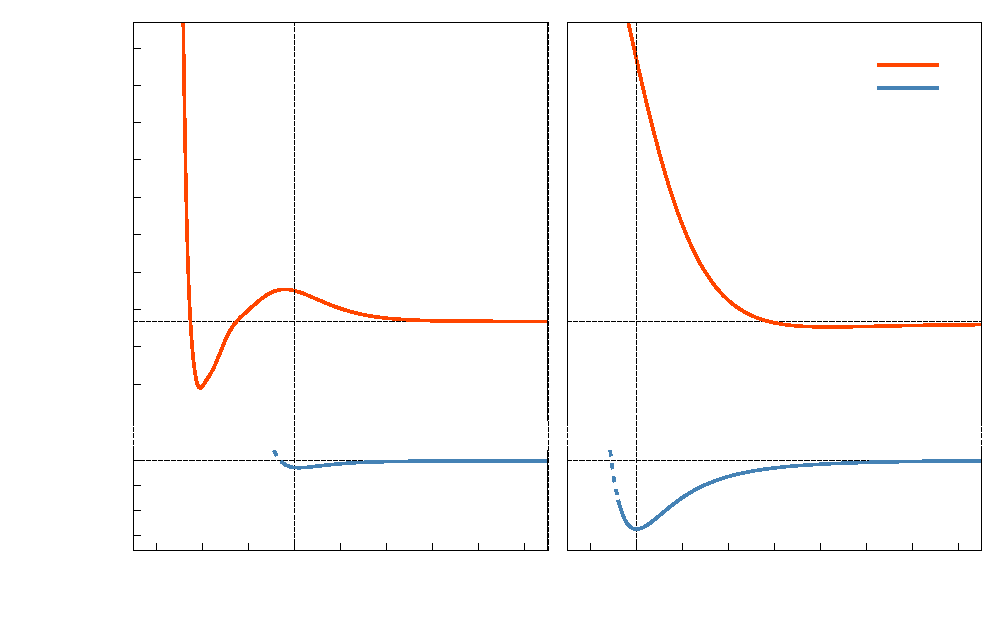
\includegraphics{DIM-5s-pot}}%
    \gplfronttext
  \end{picture}%
\endgroup

    \vspace{-0.5\baselineskip}
    \caption{Pair potential (left) and averaged interaction over the droplet (right). Equilibrium distances: $r=7.0$ \AA{} for KHe and $r=26.3$ \AA{} (between centers of mass) for KHe$_{1000}$}
    \label{fig:DIM-5s-pot}
\end{figure}
 \vspace{-1\baselineskip}
\subsubsection{An in-depth description with the ($4p$) state}
\label{sec:DIM-4p}

The ($4p$) state is more involved since it corresponds to $L=1$: on the one hand it no longer has spherical symmetry but cylindrical symmetry, and on the other hand spin-orbit coupling has to be taken into account. 
Let us first focus on the electrostatic interaction. 
\begin{align*}
U^{4p/\DIM}_{ij\alpha\beta}(\vb{r}_m) &= \bra{i,\alpha} \mathcal{R}_m^{-1} H^{4p/\DIM}_\KHE(\vb{r}_m) \, \mathcal{R}_m \ket{j,\beta} \\
&= \bra{i,\alpha} \mathcal{R}_m^{-1} \left(V^{4p}_\Pi(\vb{r}_n) \, \mathbb{I}_3 + [V^{4p}_\Sigma(\vb{r}_n) -V^{4p}_\Pi(\vb{r}_n) ]  \ket{p_{z_n}}\bra{p_{z_n}} \right) \, \mathcal{R}_m \ket{j,\beta} \\
&= \bra{i,\alpha} \left(V^{4p}_\Pi(\vb{r}_n) \, \mathbb{I}_3 + [V^{4p}_\Sigma(\vb{r}_n) -V^{4p}_\Pi(\vb{r}_n) ]   \{ \mathcal{R}_m^{-1}\ket{p_{z_n}}\bra{p_{z_n}}\mathcal{R}_m\} \right) \,  \ket{j,\beta} \num\\
&= \left(  V^{4p}_\Pi(\vb{r}_n) \, \delta_{ij}   + [V^{4p}_\Sigma(\vb{r}_n) -V^{4p}_\Pi(\vb{r}_n) ] \bra{i} \mathcal{R}_m^{-1}\ket{p_{z_n}}\bra{p_{z_n}}\mathcal{R}_m\ket{j} \right) \, \delta_{\alpha\beta}\num
\end{align*}

Expressing the interaction in a set of real orbitals makes the expression of the rotation easier because they transform as $\mathbb{R}^3$ vectors
\begin{align}
\bra{i} \mathcal{R}_m^{-1} \ket{p_{z_m}} \bra{p_{z_m}} \mathcal{R}_m \ket{j} = \frac{x^i_m \, x^j_m}{\|\vb{r}_m\|^2}
\end{align}

We can then write the electrostatic matrix elements
\begin{align}
U^{4p/\DIM}_{ij\alpha\beta}(\vb{r}_m) &= \left( V_\Pi(\vb{r}_m) \, \delta_{ij} + [V_\Sigma(\vb{r}_m) -V_\Pi(\vb{r}_m) ] \, \frac{x^i_m \, x^j_m}{\|\vb{r}_m\|^2} \right) \, \delta_{\alpha\beta} \label{eq:DIM-udef} \\
E^{4p/\DIM}_{ij\alpha\beta}(\vb{r}_\K) &= \int \dd{\vb{r}} \rho(\vb{r} + \vb{r}_\K) \, \left( V_\Pi(\vb{r}) \, \delta_{ij} + [V_\Sigma(\vb{r}) -V_\Pi(\vb{r}) ] \, \frac{x^i \, x^j}{\|\vb{r}\|^2} \right) \, \delta_{\alpha\beta}
\end{align}

Diagonalizing the electrostatic Hamiltonian within cylindrical symmetry\footnote{The ground state helium droplet being spherical, the ground state for K-He$_N$ has cylindrical symmetry, and this symmetry is conserved upon excitation.} gives a set of eigenvalues $\{ \varepsilon\}$

\begin{align*}
\varepsilon_i(\vb{r}_\K) = E^{4p/\DIM}_{ii\alpha\alpha}(\vb{r}_\K) = 2\pi \iint & r^2 \sin\theta \dd{\theta} \dd{r} \, \rho\left(\sqrt{|r^2 + r_\K^2 + 2r r_\K \cos\theta|}\right) \\
& \left( V_\Pi(r) + [V_\Sigma(r) -V_\Pi(r) ] \, \left[\frac{1}{2}(\delta_{ip_x}+\delta_{ip_y}) \sin^2\theta + \delta_{ip_z} \cos^2 \theta \right] \right) \num
\end{align*}
Because of the overall cylindrical symmetry we see that the Hamiltonian is diagonal in the common basis.
In particular the associated eigenvectors are the real $4p$-orbitals $\{ \ket{4p_{x},\pm},\ket{4p_{y},\pm},\ket{4p_{z}},\pm\}$\footnote{Note that these states are actually doubly degenerate because of spin degeneracy} and $\Lambda$ is a good quantum number. \\

We now turn to the spin-orbit interaction in the same basis set, which is known as the \textit{uncoupled} basis set: $\{\ket{p_x,+}, \ket{p_x,-}, \ket{p_y,+}, \ket{p_y,-}, \ket{p_z,+}, \ket{p_z,-} \}$. 
The matrix elements of the spin-orbit Hamiltonian are more easily expressed in the basis set of (complex) orbitals with a well defined value of $\Lambda$, and then transformed back to the real (cartesian) orbitals. We end up with

\begin{align}
H^{4p/\SO} &= A_\LS \, \vb{L}\cdot\vb{S} = A_\LS \, (L_+S_- + L_-S_+ + L_z S_z)	 
= \frac{A_\LS}{2} \mqty(	0 &  0 & -i &  0 &  0 &  1 \\
 			 				 	0 &  0 &  0 &  i & -1 &  0 \\
 			 				 	i &  0 &  0 &  0 &  0 & -i \\
 			 					0 & -i &  0 &  0 & -i &  0 \\
 								0 & -1 &  0 &  i &  0 &  0 \\
 			 					1 &  0 &  i &  0 &  0 &  0)				
\end{align}

The matrix elements of the full Hamiltonian are then
\begin{align}
U^{4p}_{ij\alpha\beta}(\vb{r}_m) &= U^{4p/\DIM}_{ij\alpha\beta}(\vb{r}_m) + U^{4p/\SO}_{ij\alpha\beta}\\
E^{4p}_{ij\alpha\beta}(\vb{r}_\K) &= \int \dd{\vb{r}} \rho(\vb{r} + \vb{r}_\K) \, \left( V_\Pi(\vb{r}) \, \delta_{ij} + [V_\Sigma(\vb{r}) -V_\Pi(\vb{r}) ] \, \frac{x^i \, x^j}{\|\vb{r}\|^2} \right) \, \delta_{\alpha\beta} + U^{4p/\SO}_{ij\alpha\beta} \\
\end{align}

Its diagonalization gives the set of eigenvalues $\{\xi\}$
\begin{align*}
\xi_1(\vb{r}_\K) &= \frac{1}{2} (\varepsilon_1 + \varepsilon_3) + \frac{1}{4}\left(-A_\LS+\sqrt{9 A_\LS^2-4 A_\LS(\varepsilon_1-\varepsilon_3) + 4(\varepsilon_1-\varepsilon_3)^2}\right) \\		
\xi_2(\vb{r}_\K) &= \varepsilon_1 + \frac{A_\LS}{2} \label{eq:DIM-SO-nrj} \num \\
\xi_3(\vb{r}_\K) &= \frac{1}{2} (\varepsilon_1 + \varepsilon_3) + \frac{1}{4}\left(-A_\LS-\sqrt{9 A_\LS^2-4 A_\LS(\varepsilon_1-\varepsilon_3) + 4(\varepsilon_1-\varepsilon_3)^2}\right)
\end{align*}

\begin{table}[!h]
\centering
\begin{tabular}{|c|c|c|c|}
\hline
 & $\xi_1$ & $\xi_2$ & $\xi_3$  \\
\hline
Value when $\varepsilon_i \ll A_\LS$ & $+\frac{A_\LS}{2}$ & $+\frac{A_\LS}{2}$ & $-A_\LS$\\  
\hline
Associated $J$ value & $3/2$ & $3/2$ & $1/2$\\  
\hline
Value when $\varepsilon_i \gg A_\LS$ & $\varepsilon_3$ & $\varepsilon_1$ & $\varepsilon_1$ \\
\hline
Associated $|\Lambda|$ value & $0$ & $1$  & $1$  \\
\hline
Associated $|\Omega|$ value & $1/2$ & $3/2$ & $1/2$ \\
\hline
Label & $\Sigma_{1/2}$ & $\Pi_{3/2}$ & $ \Pi_{1/2}$ \\
\hline
\end{tabular}
\caption{Determination of true good quantum number $\Omega$ and approximate ones $\Lambda$ and $J$}
\label{table:DIM-labels}
\end{table}

\begin{figure}[h!]
\centering
    % GNUPLOT: LaTeX picture with Postscript
\begingroup
  \makeatletter
  \providecommand\color[2][]{%
    \GenericError{(gnuplot) \space\space\space\@spaces}{%
      Package color not loaded in conjunction with
      terminal option `colourtext'%
    }{See the gnuplot documentation for explanation.%
    }{Either use 'blacktext' in gnuplot or load the package
      color.sty in LaTeX.}%
    \renewcommand\color[2][]{}%
  }%
  \providecommand\includegraphics[2][]{%
    \GenericError{(gnuplot) \space\space\space\@spaces}{%
      Package graphicx or graphics not loaded%
    }{See the gnuplot documentation for explanation.%
    }{The gnuplot epslatex terminal needs graphicx.sty or graphics.sty.}%
    \renewcommand\includegraphics[2][]{}%
  }%
  \providecommand\rotatebox[2]{#2}%
  \@ifundefined{ifGPcolor}{%
    \newif\ifGPcolor
    \GPcolortrue
  }{}%
  \@ifundefined{ifGPblacktext}{%
    \newif\ifGPblacktext
    \GPblacktextfalse
  }{}%
  % define a \g@addto@macro without @ in the name:
  \let\gplgaddtomacro\g@addto@macro
  % define empty templates for all commands taking text:
  \gdef\gplbacktext{}%
  \gdef\gplfronttext{}%
  \makeatother
  \ifGPblacktext
    % no textcolor at all
    \def\colorrgb#1{}%
    \def\colorgray#1{}%
  \else
    % gray or color?
    \ifGPcolor
      \def\colorrgb#1{\color[rgb]{#1}}%
      \def\colorgray#1{\color[gray]{#1}}%
      \expandafter\def\csname LTw\endcsname{\color{white}}%
      \expandafter\def\csname LTb\endcsname{\color{black}}%
      \expandafter\def\csname LTa\endcsname{\color{black}}%
      \expandafter\def\csname LT0\endcsname{\color[rgb]{1,0,0}}%
      \expandafter\def\csname LT1\endcsname{\color[rgb]{0,1,0}}%
      \expandafter\def\csname LT2\endcsname{\color[rgb]{0,0,1}}%
      \expandafter\def\csname LT3\endcsname{\color[rgb]{1,0,1}}%
      \expandafter\def\csname LT4\endcsname{\color[rgb]{0,1,1}}%
      \expandafter\def\csname LT5\endcsname{\color[rgb]{1,1,0}}%
      \expandafter\def\csname LT6\endcsname{\color[rgb]{0,0,0}}%
      \expandafter\def\csname LT7\endcsname{\color[rgb]{1,0.3,0}}%
      \expandafter\def\csname LT8\endcsname{\color[rgb]{0.5,0.5,0.5}}%
    \else
      % gray
      \def\colorrgb#1{\color{black}}%
      \def\colorgray#1{\color[gray]{#1}}%
      \expandafter\def\csname LTw\endcsname{\color{white}}%
      \expandafter\def\csname LTb\endcsname{\color{black}}%
      \expandafter\def\csname LTa\endcsname{\color{black}}%
      \expandafter\def\csname LT0\endcsname{\color{black}}%
      \expandafter\def\csname LT1\endcsname{\color{black}}%
      \expandafter\def\csname LT2\endcsname{\color{black}}%
      \expandafter\def\csname LT3\endcsname{\color{black}}%
      \expandafter\def\csname LT4\endcsname{\color{black}}%
      \expandafter\def\csname LT5\endcsname{\color{black}}%
      \expandafter\def\csname LT6\endcsname{\color{black}}%
      \expandafter\def\csname LT7\endcsname{\color{black}}%
      \expandafter\def\csname LT8\endcsname{\color{black}}%
    \fi
  \fi
    \setlength{\unitlength}{0.0500bp}%
    \ifx\gptboxheight\undefined%
      \newlength{\gptboxheight}%
      \newlength{\gptboxwidth}%
      \newsavebox{\gptboxtext}%
    \fi%
    \setlength{\fboxrule}{0.5pt}%
    \setlength{\fboxsep}{1pt}%
\begin{picture}(9360.00,5760.00)%
    \gplgaddtomacro\gplbacktext{%
      \csname LTb\endcsname%
      \put(991,1877){\makebox(0,0)[r]{\strut{}$18350$}}%
      \put(991,2259){\makebox(0,0)[r]{\strut{}$18400$}}%
      \put(991,2642){\makebox(0,0)[r]{\strut{}$18450$}}%
      \put(991,3024){\makebox(0,0)[r]{\strut{}$18500$}}%
      \put(991,3407){\makebox(0,0)[r]{\strut{}$18550$}}%
      \put(991,3789){\makebox(0,0)[r]{\strut{}$18600$}}%
      \put(991,4171){\makebox(0,0)[r]{\strut{}$18650$}}%
      \put(991,4554){\makebox(0,0)[r]{\strut{}$18700$}}%
      \put(991,4936){\makebox(0,0)[r]{\strut{}$18750$}}%
      \put(991,5319){\makebox(0,0)[r]{\strut{}$18800$}}%
      \put(991,5701){\makebox(0,0)[r]{\strut{}$18850$}}%
      \put(199,3167){\rotatebox{90}{\makebox(0,0){\strut{}Energy (K)}}}%
      \put(5194,149){\makebox(0,0){\strut{}Distance from equilibrium position (\AA)}}%
    }%
    \gplgaddtomacro\gplfronttext{%
      \csname LTb\endcsname%
      \put(8260,3210){\makebox(0,0)[r]{\strut{}$\Pi_{1/2}$}}%
      \csname LTb\endcsname%
      \put(8260,2990){\makebox(0,0)[r]{\strut{}$\Pi_{3/2}$}}%
      \csname LTb\endcsname%
      \put(8260,2770){\makebox(0,0)[r]{\strut{}$\Sigma_{1/2}$}}%
      \csname LTb\endcsname%
      \put(8260,2550){\makebox(0,0)[r]{\strut{}4s}}%
    }%
    \gplgaddtomacro\gplbacktext{%
      \csname LTb\endcsname%
      \put(991,776){\makebox(0,0)[r]{\strut{}$-15$}}%
      \put(991,1015){\makebox(0,0)[r]{\strut{}$-10$}}%
      \put(991,1254){\makebox(0,0)[r]{\strut{}$-5$}}%
      \put(991,1493){\makebox(0,0)[r]{\strut{}$0$}}%
      \put(1123,413){\makebox(0,0){\strut{}$-6$}}%
      \put(1735,413){\makebox(0,0){\strut{}$-4$}}%
      \put(2347,413){\makebox(0,0){\strut{}$-2$}}%
      \put(2959,413){\makebox(0,0){\strut{}$0$}}%
      \put(3570,413){\makebox(0,0){\strut{}$2$}}%
      \put(4182,413){\makebox(0,0){\strut{}$4$}}%
      \put(4794,413){\makebox(0,0){\strut{}$6$}}%
    }%
    \gplgaddtomacro\gplfronttext{%
    }%
    \gplgaddtomacro\gplbacktext{%
    }%
    \gplgaddtomacro\gplfronttext{%
    }%
    \gplgaddtomacro\gplbacktext{%
      \csname LTb\endcsname%
      \put(5441,413){\makebox(0,0){\strut{}$-2$}}%
      \put(6053,413){\makebox(0,0){\strut{}$0$}}%
      \put(6665,413){\makebox(0,0){\strut{}$2$}}%
      \put(7277,413){\makebox(0,0){\strut{}$4$}}%
      \put(7888,413){\makebox(0,0){\strut{}$6$}}%
      \put(8500,413){\makebox(0,0){\strut{}$8$}}%
      \put(9112,413){\makebox(0,0){\strut{}$10$}}%
    }%
    \gplgaddtomacro\gplfronttext{%
    }%
    \gplbacktext
    \put(0,0){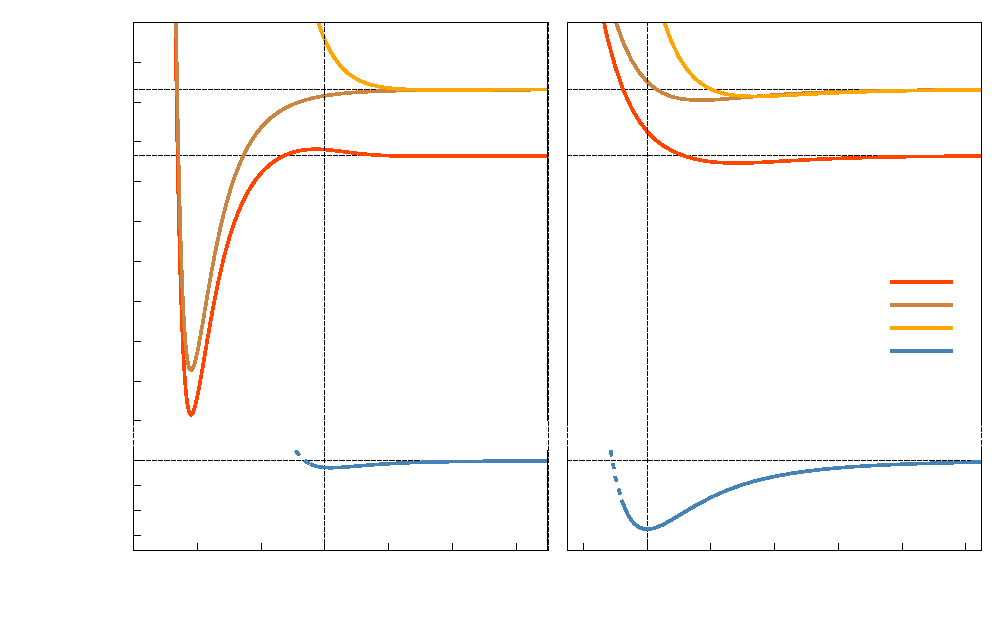
\includegraphics{DIM-p-pot}}%
    \gplfronttext
  \end{picture}%
\endgroup

    \vspace{-0.5\baselineskip}
    \caption{Pair potential (left) and averaged interaction over the droplet (right)}
    \label{fig:DIM-4p-pot}
\end{figure}

We present in \cittab{table:DIM-labels} the reasoning used to determine the true good quantum number $\Omega$ and the approximate ones: $\Lambda$ and $J$. 
We use the following label $\Lambda_\Omega$ for energy states. % (Hund's case (a) for coupling of angular momenta).
$J$ does not appear because in the excitation region the $\Sigma-\Pi$ splitting between electrostatic eigenvalues is larger that the atomic spin-orbit splitting, such that $\Lambda$ gives a better representation of the reality.\\

In the same way than for the ($5s$) state (\citfig{fig:DIM-5s-pot}), we plot both the pair interaction and the averaged potential in \citfig{fig:DIM-4p-pot}. Keep in mind that pair potential refers to the unrotated basis, for instance in a global $\Pi_{1/2}$ state, there are only the helium in the internuclear axis that interact with $\Pi_{1/2}$ potential. Note also that the averaged potential corresponds to one of the $\xi$ value labeled according to the previous discussion.

\subsection{Writing energy contribution to doped helium droplet}

In order to describe the electronic degree of freedom, we introduce the electronic wave function $\ket{\lambda}$
\begin{align}
\ket{\lambda} = \sum_{\underset{i\in \{nl \, \text{orbitals}\}}{\alpha=\{+,-\}}} \lambda_{i\alpha} \ket{i,\alpha}
\label{eq:DIM-lambda-state}
\end{align}

Let us consider the interaction Hamiltonian for $H^{nl}_\KHEN(\vb{r}_\K)$ (\citeq{eq:DIM-hamtot}), we will write the corresponding interaction in the continuum formalism. 
We first describe the total energy for a point-like interaction, \textit{id est} a classical particle
\begin{align}
E[\rho] \rightarrow E[\rho, \vb{r}_\K,\lambda] &= E[\rho]  + \bra{\Psi,\lambda}H^{nl}_\KHEN(\vb{r}_\K)\ket{\Psi,\lambda} \label{eq:DIM-C-nrj-correction}
\end{align}
The interaction part is given by
\begin{align}
\bra{\Psi,\lambda}H^{nl}_\KHEN\ket{\Psi,\lambda} &= \int \dd{\vb{r}} \, \rho(\vb{r}+\vb{r}_\K) \bra{\lambda} \mathcal{R}^{-1}(\vb{r}) H^{nl/\DIM}_\KHE(\vb{r}) \, \mathcal{R}(\vb{r})\ket{\lambda} + \bra{\lambda}H^{nl/\SO} \ket{\lambda}\\
&\equiv \int \dd{\vb{r}} \, \rho(\vb{r}) \, V_\KHE^{nl\lambda}(\vb{r}-\vb{r}_\K) +  \bra{\lambda}H^{nl/\SO} \ket{\lambda}
\end{align}
where the time evolution of the \emph{effective} potential is given by that of the electronic wave packet $\ket{\lambda}$, using notation of \citeq{eq:DIM-udef}
\begin{align}
V_\KHE^{nl\lambda}(\vb{r}) &= \bra{\lambda} \mathcal{R}^{-1}(\vb{r}) H^{nl/\DIM}_\KHE(\vb{r}) \, \mathcal{R}(\vb{r})\ket{\lambda} =  \sum_{ij\alpha\beta} \lambda_{i\alpha}^* \, U^{nl/\DIM}_{ij\alpha\beta}(\vb{r}) \, \lambda_{j\beta}
\end{align}

For a quantum particle described by a wave function $\phi$, \citeq{eq:DIM-C-nrj-correction} becomes
\begin{align}
E[\rho] \rightarrow E[\rho, \phi,\lambda] &= E[\rho]  + \bra{\Psi,\lambda, \phi}H^{nl}_\KHEN(\vb{r}_\K)\ket{\Psi,\lambda, \phi}
\end{align}

In the classical case, variation of the total energy with respect to the effective helium wave function (order parameter) $\Psi$ gives the \textsc{Euler-Lagrange} equations.

\begin{align}
&E[\rho,\vb{r}_\K,\lambda] = E[\rho] + \int \dd{\vb{r}} \, \rho(\vb{r}) V^{nl\lambda}_\KHE(\vb{r}-\vb{r}_\K) + \bra{\lambda}H^{nl/\SO}\ket{\lambda} \\
&\Rightarrow \left( -\frac{\hbar^2}{2m_\K} \grad{}^2 + \frac{\delta \mathcal{E}_c}{\delta \rho} + V^{nl\lambda}_\KHE(\vb{r}-\vb{r}_\K)\right)\Psi(\vb{r})=\mu \Psi(\vb{r})
\end{align}

In the quantum case one adds variation with respect to the alkali wave function, which yields two coupled equations
\begin{align*}
&E[\rho,\phi,\lambda] = E[\rho] + \iint \dd{\vb{r}}\dd{\vb{r}_\K} \, \rho(\vb{r}) V^{nl\lambda}_\KHE(\vb{r}-\vb{r}_\K) |\phi(\vb{r}_\K)|^2 \\
& \qquad \qquad \qquad \qquad \qquad \qquad \qquad + \frac{\hbar^2}{2m_\K} \int \dd{\vb{r}_\K} |\grad{}_{\vb{r}_\K}\phi(\vb{r}_\K)|^2 + \bra{\lambda}H^{nl/\SO}\ket{\lambda} \num \\
&\Rightarrow \left\{
\begin{array}{l}
  \left( -\frac{\hbar^2}{2m_\HE} \grad{}_{\vb{r}}^2 + \frac{\delta \mathcal{E}_c}{\delta \rho} + \int \dd{\vb{r}_\K} \,V^{nl\lambda}_\KHE(\vb{r}-\vb{r}_\K)|\phi(\vb{r}_\K)|^2 \right)\Psi(\vb{r})=\mu \Psi(\vb{r})\\
\left( -\frac{\hbar^2}{2m_\K} \grad{}_{\vb{r}_\K}^2 + \int \dd{\vb{r}} \,V^{nl\lambda}_\KHE(\vb{r}-\vb{r}_\K)\rho(\vb{r}) \right)\phi(\vb{r}_\K)=\varepsilon \phi(\vb{r}_\K)
\end{array}
\right. \num 
\end{align*}

We see that thanks to the introduction of the \textit{order parameter} these equations look like \textsc{Schrodinger} equations.
Technical details on how to solve these equations are given in the \citanx{sec:ANX-itp}.
